\section{Conditional Distributions and Joint Continuity}

\subsection{Joint PMF of Discrete Random Variables}

If \( X \) and \( Y \) are discrete random variables, the range of the mapping \( (X(\cdot), Y(\cdot)) \) forms a countable subset of \( \mathbb{R}^2 \). This arises from the fact that the Cartesian product of two countable sets is also countable. To clarify, a set is considered countable if it can be put into a one-to-one correspondence with the natural numbers. Therefore, since both \( X \) and \( Y \) take on countably many values, their combined behavior represented by \( (X, Y) \) will also be countable, thus making \( (X(\cdot), Y(\cdot)) \) a discrete random variable on \( \mathbb{R}^2 \).\\

It's important to note that we cannot make the same assertion when \( X \) and \( Y \) are continuous random variables. In such cases, even if \( X \) and \( Y \) are each continuous on their own, they may not be jointly continuous. Refer subsection 4.5.3 for this. \\

The joint probability mass function (pmf) of the discrete random variables \( X \) and \( Y \) is given by:

\[
p_{X,Y}(x, y) = P(X = x, Y = y), \quad x, y \in \mathbb{R}.
\]

This joint pmf plays a crucial role in defining the joint distribution of \( X \) and \( Y \). Specifically, for any Borel set \( B \in \mathcal{B}_{\mathbb{R}^2} \), the probability that the random vector \( (X, Y) \) falls within the set \( B \) is given by:

\[
P_{X,Y}(B) = \sum_{(x,y) \in B} p_{X,Y}(x, y).
\]

This equation shows that the joint pmf allows us to calculate probabilities associated with any region in the plane defined by the variables \( X \) and \( Y \).


\subsection{Conditional PMF of Discrete Random Variables}

Now, we define the conditional probability mass function (pmf) for discrete random variables.\\

\begin{definition}
    Let \(X\) and \(Y\) be discrete random variables defined on the probability space \((\Omega, \mathcal{F}, P)\). The conditional probability of \(X\) given \(Y\) is defined as:

\[
p_{X|Y}(x|y) = P(X = x | Y = y) = \frac{P(X = x, Y = y)}{P(Y = y)} = \frac{p_{X,Y}(x, y)}{p_Y(y)}
\]

where \(p_Y(y) > 0\).
\end{definition}

The following theorem describes the concept of independence for discrete random variables in terms of the conditional pmf.

\begin{theorem}
    The following statements are equivalent for discrete random variables \(X\) and \(Y\):\\

1. \(X\) and \(Y\) are independent.\\
2. For all \(x, y \in \mathbb{R}\), the events \(\{X = x\}\) and \(\{Y = y\}\) are independent.\\
3. For all \(x, y \in \mathbb{R}\), \(P_{X,Y}(x, y) = P_X(x)P_Y(y)\).\\
4. For all \(x, y \in \mathbb{R}\) such that \(p_Y(y) > 0\), \(p_{X|Y}(x|y) = p_X(x)\).
`'
\end{theorem}

\begin{proof}
    
The equivalences (2) $\Leftrightarrow$ (3) and (3) $\Leftrightarrow$ (4) follow directly from the definitions of independence and the conditional pmf. \\

Now, let us prove the equivalence between (1) and (3):\\

\textbf{(1) implies (3):} If \(X\) and \(Y\) are independent, then the joint probability of \(X\) and \(Y\) can be expressed as:

\[
P(X \in B_1, Y \in B_2) = P(X \in B_1) P(Y \in B_2).
\]

Now, let \(B_1 = \{x\}\) and \(B_2 = \{y\}\). Therefore, we have:

\[
P(X = x, Y = y) = P(X = x) P(Y = y).
\]

This establishes statement (3).\\

\textbf{(3) implies (1):} Given that \(P(X \in B_1, Y \in B_2) = P_{X,Y}(x,y)\), we can write:

\[
P(X \in B_1, Y \in B_2) = \sum_{x \in B_1} \sum_{y \in B_2} p_{X,Y}(x, y).
\]

Using statement (3), we substitute to obtain:

\[
\sum_{x \in B_1} \sum_{y \in B_2} P_X(x) P_Y(y) = \sum_{x \in B_1} P_X(x) \sum_{y \in B_2} P_Y(y) = P(X \in B_1) P(Y \in B_2).
\]

This confirms statement (1). Thus, we have shown that the statements are equivalent.
\end{proof}

\subsection{Joint PMF of Continuous Random Variables}

\begin{definition}
    Two random variables \( X \) and \( Y \) are termed \textit{jointly continuous} if their joint probability distribution, denoted \( P_{X,Y} \), is absolutely continuous with respect to the Lebesgue measure on \( \mathbb{R}^2 \). This means that for every Borel set \( N \subset \mathbb{R}^2 \) with Lebesgue measure zero, we have:
    \[
    P((X, Y) \in N) = 0.
    \]
\end{definition}

In simple terms, this ensures that there is no \textit{mass} of probability concentrated on any set of points with zero area in \( \mathbb{R}^2 \). For \( X \) and \( Y \) to be jointly continuous, their probability distribution must spread smoothly over regions in \( \mathbb{R}^2 \), without \textit{spikes} or \textit{isolated points.}\\

The \textit{Radon-Nikodym Theorem} gives us a more practical tool here. 

\begin{theorem}
    \( X \) and \( Y \) are jointly continuous random variables if and only if there exists a measurable function \( f_{X,Y} : \mathbb{R}^2 \to [0, \infty) \), called the \textit{joint probability density function} (pdf), such that for any region \( B \subset \mathbb{R}^2 \),
    \[
    P((X, Y) \in B) = \int_{B} f_{X,Y}(u, v) \, d\lambda(u, v),
    \]
    where \( \lambda \) represents the Lebesgue measure on \( \mathbb{R}^2 \).
\end{theorem}

\textbf{Implication of Joint Continuity}: To express this in a familiar form, let’s examine the probability that \( X \) and \( Y \) fall within certain ranges. For \( B = (-\infty, x] \times (-\infty, y] \), this probability becomes:
\[
F_{X,Y}(x, y) = P(X \leq x, Y \leq y) = \int_{-\infty}^{x} \int_{-\infty}^{y} f_{X,Y}(u, v) \, dv \, du,
\]
where \( F_{X,Y}(x, y) \) is the \textit{joint cumulative distribution function} (cdf), and \( f_{X,Y}(x, y) \) is the \textit{joint pdf}. \\

Thus, the joint pdf \( f_{X,Y}(x, y) \) provides a complete description of the joint behavior of \( X \) and \( Y \). This means that knowing \( f_{X,Y}(x, y) \) allows us to compute the probabilities for any event involving \( X \) and \( Y \) over regions in \( \mathbb{R}^2 \). \\

\begin{lemma}
    If \( X \) is continuous and \( Y \) is continuous, then \((X, Y)\) need not be jointly continuous.
\end{lemma}

We won't formally prove this lemma, but we will provide an example that confirms that this is true. 

\begin{example}
    Suppose \( X \sim N(0, 1) \), meaning that \( X \) is a standard normal random variable with mean \( 0 \) and variance \( 1 \), and \( Y = 2X \). So, \( Y \) will have a mean of \( 0 \) and a variance of \( 4 \), which we can verify by noting that
\[
Y \sim N(0, 4).
\]

Even though both \( X \) and \( Y \) are continuous random variables, we need to examine if they form a jointly continuous pair when taken together as the random vector \( (X, Y) \).\\

A pair of random variables \( (X, Y) \) is considered jointly continuous if there exists a joint probability density function \( f_{X,Y}(x, y) \) over the entire \( \mathbb{R}^2 \) space, such that for any subset \( A \subset \mathbb{R}^2 \),
\[
P((X, Y) \in A) = \iint_A f_{X,Y}(x, y) \, dx \, dy.
\]

Notice that \( Y = 2X \) directly ties \( Y \) to \( X \). This means \( Y \) is perfectly linearly dependent on \( X \), implying that \( (X, Y) \) does not vary freely across the \( \mathbb{R}^2 \) plane. Instead, the values of \( (X, Y) \) are restricted to a specific line, namely \( y = 2x \). Since \( Y = 2X \), the pair \( (X, Y) \) essentially lies along the line \( y = 2x \) in the \( \mathbb{R}^2 \) plane. Consequently, the joint probability measure of \( (X, Y) \) is concentrated along this line rather than spread across two dimensions.\\ 

In terms of probability density, this restriction means that there does not exist a two-dimensional joint density \( f_{X,Y}(x, y) \) over the entire \( \mathbb{R}^2 \) space, because we cannot assign probabilities over regions in \( \mathbb{R}^2 \) outside this line. Any density that would describe \( (X, Y) \) is confined to one dimension along \( y = 2x \).\\


Thus, although \( X \) and \( Y \) are individually continuous, \( (X, Y) \) as a pair does not possess joint continuity in two dimensions.
\end{example}

\begin{lemma}
    When \( X \) and \( Y \) are jointly continuous random variables, their marginal distributions are also continuous. To understand why, let’s examine the probability that \( X \leq x \) and \( Y \leq y \):
\[
P(X \leq x, Y \leq y) = \int_{-\infty}^{x} \int_{-\infty}^{y} f_{X,Y}(u, v) \, dv \, du
\]
\end{lemma}


Now, we want to find the marginal distribution of \( X \). The marginal probability \( P(X \leq x) \) is obtained by integrating over all possible values of \( Y \):

\[
P(X \leq x) = \int_{-\infty}^{x} \left( \int_{-\infty}^{\infty} f_{X,Y}(u, v) \, dv \right) du = \int_{-\infty}^{x} f_X(u) \, du
\]

Here, the expression inside the parentheses,

\[
\int_{-\infty}^{\infty} f_{X,Y}(u, v) \, dv,
\]

produces a function of \( u \) which is non-negative and measurable. This function represents the density of \( X \), which we denote as \( f_X(u) \). \\

Thus, we can write:

\[
f_X(u) = \int_{-\infty}^{\infty} f_{X,Y}(u, v) \, dv
\]

This shows that \( X \) has a continuous marginal distribution with \( f_X \) as its probability density function (pdf). Since \( f_X(u) \) is derived as an integral over a non-negative function \( f_{X,Y}(u, v) \), it ensures that \( f_X \) itself is also non-negative and measurable.\\

A similar argument applies to the marginal pdf of \( Y \), confirming that both \( X \) and \( Y \) are indeed continuous. This continuity of the marginals follows directly from the joint continuity of \( X \) and \( Y \), as we have shown through their integrals.

\begin{definition}
    \textbf{Independence of Joint Continuous Random Variables.} For two random variables \( X \) and \( Y \), we say they are \textbf{independent} if and only if their joint distribution function \( F_{X,Y}(x, y) \) can be written as the product of their marginal distribution functions. In other words, 

    \[
    F_{X,Y}(x, y) = F_X(x) F_Y(y) \quad \forall x, y \in \mathbb{R}.
    \]
\end{definition}

Now, let's apply this definition to a specific case: when \( X \) and \( Y \) are \textbf{jointly continuous} random variables. For continuous variables, we express independence in terms of their probability density functions. That is, we integrate the joint density function \( f_{X,Y}(x, y) \) over the range \((-\infty, x]\) and \((-\infty, y]\):

\[
\int_{-\infty}^{x} \int_{-\infty}^{y} f_{X,Y}(u, v) \, dv \, du = 
\left( \int_{-\infty}^{x} f_X(u) \, du \right) \left( \int_{-\infty}^{y} f_Y(v) \, dv \right).
\]

Expanding this, we see that independence requires

\[
\int_{-\infty}^{x} \int_{-\infty}^{y} f_{X,Y}(u, v) \, dv \, du = \int_{-\infty}^{x} \int_{-\infty}^{y} f_X(u) f_Y(v) \, dv \, du.
\]

Since this equality holds for \textit{all} values of \( x \) and \( y \), we can conclude that the two integrands themselves must be equal almost everywhere. Therefore,

\[
f_{X,Y}(x, y) = f_X(x) f_Y(y) \quad \forall x, y \in \mathbb{R},
\]

except possibly on a subset of \( \mathbb{R}^2 \) with Lebesgue measure zero. This condition—that the joint density factorizes as the product of the marginal densities—is both a \textbf{necessary and sufficient condition} for the independence of two jointly continuous random variables.

\subsection{Conditional PDF of Continuous Random Variables}

To define the conditional cumulative distribution function (CDF) \( F_{X|Y}(x | y) \approx P(X \leq x | Y = y) \), we face a technical challenge: the event \( \{ Y = y \} \) has probability zero for any specific \( y \) when \( Y \) is a continuous random variable. This zero-probability event makes a direct conditional probability definition problematic.\\

To resolve this, we approximate by conditioning on \( Y \) taking values within a small interval \( (y, y + \epsilon) \), where \( \epsilon > 0 \). We then examine what happens as \( \epsilon \) approaches zero. This approach leads to a motivating derivation for defining the conditional probability density function (pdf) in the jointly continuous case.\\

The conditional CDF of \( X \), given that \( Y \) is \textit{close to \( y \),} can be approximated by:
\[
F_{X|Y}(x | y) = P(X \leq x \mid y \leq Y \leq y + \epsilon) \quad \text{(for small } \epsilon \text{)}.
\]
This probability can be rewritten in terms of joint and marginal probabilities as:
\[
F_{X|Y}(x | y) = \frac{P(\{ X \leq x \} \cap \{ y \leq Y \leq y + \epsilon \})}{P(y \leq Y \leq y + \epsilon)}.
\]
To express this in terms of CDFs, we observe that:
\[
F_{X|Y}(x | y) = \frac{F_{X,Y}(x, y + \epsilon) - F_{X,Y}(x, y)}{F_{Y}(y + \epsilon) - F_{Y}(y)}.
\]
Now, dividing the numerator and denominator by \( \epsilon \), we obtain:
\[
F_{X|Y}(x | y) = \frac{\frac{F_{X,Y}(x, y + \epsilon) - F_{X,Y}(x, y)}{\epsilon}}{\frac{F_{Y}(y + \epsilon) - F_{Y}(y)}{\epsilon}}.
\]
As \( \epsilon \to 0 \), the right-hand side of this expression resembles the form of a derivative. Specifically, it suggests:
\[
F_{X|Y}(x | y) = \frac{\frac{\partial}{\partial y} F_{X,Y}(x, y)}{\frac{d}{d y} F_{Y}(y)}.
\]
This expression provides a foundation for defining the conditional CDF and, by extension, the conditional PDF.


\begin{definition}
    The \textbf{conditional cumulative distribution function} (CDF) of a random variable \( X \) given \( Y = y \) is a way to accumulate probability up to a certain point \( x \), while taking into account the information provided by \( Y = y \). It is defined as:
   \[
   F_{X|Y}(x | y) = \int_{-\infty}^{x} \frac{f_{X,Y}(u, y)}{f_Y(y)} \, du,
   \]
   where \( f_{X,Y}(u, y) \) is the joint probability density function (pdf) of \( X \) and \( Y \), and \( f_Y(y) \) is the marginal pdf of \( Y \). 
\end{definition}

Note that this expression is valid as long as \( f_Y(y) > 0 \), since we cannot condition on an impossible or zero-probability event.

\begin{definition}
    The \textbf{conditional probability density function} (pdf) of \( X \) given \( Y = y \) tells us the probability density of \( X \) at a particular point \( x \), assuming \( Y = y \). It is defined as:
    \[
    f_{X|Y}(x | y) = \frac{f_{X,Y}(x, y)}{f_Y(y)},
    \]
    again, assuming \( f_Y(y) > 0 \).
\end{definition}

This expression gives us a way to interpret \( X \) as a function of the specific value \( y \) of \( Y \), concentrating our attention on the values \( X \) takes when \( Y = y \).

\begin{definition}
    Suppose we have an event \( A \) that belongs to the Borel \(\sigma\)-algebra \( \mathcal{B}(\mathbb{R}) \) (denoted \( A \in \mathcal{B}(\mathbb{R}) \), the collection of all Borel subsets of \( \mathbb{R} \)). The \textbf{conditional probability} of the event \( A \) given \( Y = y \) is defined as:
   \[
   P(X \in A | Y = y) = \int_{A} f_{X|Y}(v | y) \, dv = \int_{-\infty}^{\infty} \mathbb{I}_A(v) f_{X|Y}(v | y) \, dv,
   \]
   where \( \mathbb{I}_A(v) \) is the indicator function for the set \( A \), which is 1 if \( v \in A \) and 0 otherwise.
\end{definition}

This integral sums up the conditional pdf \( f_{X|Y}(v | y) \) over the region defined by \( A \), thereby giving the probability that \( X \) lies in \( A \), under the condition that \( Y = y \).


\begin{exercise}
Consider random variables \( X \) and \( Y \) with a joint continuous distribution defined over a triangular region with vertices at points \( (0, 0) \), \( (0, 2) \), and \( (1, 0) \). The joint probability density function is given by:
\[
f_{X,Y}(x, y) = 1
\]
for \((x, y)\) within the triangular region. Find the marginal distributions \( f_X(x) \) and \( f_Y(y) \), and the conditional distributions \( f_{Y|X}(y|x) \) and \( f_{X|Y}(x|y) \).\\

\begin{center}
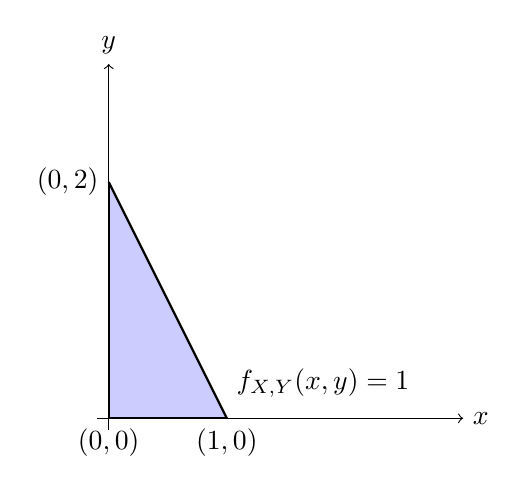
\begin{tikzpicture}[scale=1.5]
    % Draw axes
    \draw[->] (-0.1, 0) -- (3, 0) node[right] {$x$};
    \draw[->] (0, -0.1) -- (0, 3) node[above] {$y$};

    % Draw the triangular region
    \fill[blue!20] (0, 0) -- (0, 2) -- (1, 0) -- cycle;

    % Draw the edges of the triangle
    \draw[thick] (0, 0) -- (0, 2) node[above,left] {$(0, 2)$};
    \draw[thick] (0, 2) -- (1, 0) node[below, below] {$(1, 0)$};
    \draw[thick] (1, 0) -- (0, 0) node[left,below] {$(0, 0)$};

    % Add a label for the area
    \node[below right] at (1, 0.5) {$f_{X,Y}(x,y) = 1$};
\end{tikzpicture}
\end{center}

\end{exercise}

\begin{solution}
The region where \( f_{X,Y}(x, y) = 1 \) is the triangle with vertices \( (0, 0) \), \( (0, 2) \), and \( (1, 0) \). The line connecting \( (0, 2) \) and \( (1, 0) \) has the equation:
    \[
    y = 2 - 2x
    \]
    Therefore, the joint distribution \( f_{X,Y}(x, y) = 1 \) is defined for \( 0 \leq x \leq 1 \) and \( 0 \leq y \leq 2 - 2x \).\\

To ensure \( f_{X,Y}(x, y) = 1 \) is a valid probability density function, we need:
    \[
    \int_0^1 \int_0^{2 - 2x} 1 \, dy \, dx = 1
    \]
    Compute this integral:
    \[
    \int_0^1 \int_0^{2 - 2x} 1 \, dy \, dx = \int_0^1 (2 - 2x) \, dx = \int_0^1 2 - 2x \, dx = \left[ 2x - x^2 \right]_0^1 = 2 - 1 = 1
    \]
    Thus, \( f_{X,Y}(x, y) = 1 \) is indeed normalized.\\

To find \( f_X(x) \), integrate \( f_{X,Y}(x, y) \) over \( y \):
    \[
    f_X(x) = \int_0^{2 - 2x} 1 \, dy = 2 - 2x
    \]
    for \( 0 \leq x \leq 1 \).\\

To find \( f_Y(y) \), integrate \( f_{X,Y}(x, y) \) over \( x \). Note that for a given \( y \), \( x \) ranges from \( 0 \) to \( 1 - \frac{y}{2} \) (from the line equation rearranged):
    \[
    f_Y(y) = \int_0^{1 - \frac{y}{2}} 1 \, dx = 1 - \frac{y}{2}
    \]
    for \( 0 \leq y \leq 2 \).\\

The conditional distribution \( f_{Y|X}(y|x) \) is given by:
    \[
    f_{Y|X}(y|x) = \frac{f_{X,Y}(x, y)}{f_X(x)} = \frac{1}{2 - 2x}
    \]
    for \( 0 \leq y \leq 2 - 2x \).\\

The conditional distribution \( f_{X|Y}(x|y) \) is given by:
    \[
    f_{X|Y}(x|y) = \frac{f_{X,Y}(x, y)}{f_Y(y)} = \frac{1}{1 - \frac{y}{2}}
    \]
    for \( 0 \leq x \leq 1 - \frac{y}{2} \).

\end{solution}


\begin{exercise}
Two persons X and Y live in cities A and B but work in cities B and A respectively. Every morning they start for work at a uniformly random time between 9 am and 10 am independent of each other. Both of them travel at the same constant speed and it takes 20 minutes to reach the other city. What is the probability that X and Y meet each other on their way to work?
\end{exercise}

\begin{solution}
Let \( T_X \) and \( T_Y \) be the times at which persons X and Y leave their respective cities. Both \( T_X \) and \( T_Y \) are uniformly distributed over the interval \([0, 60]\) minutes, where 0 corresponds to 9:00 am and 60 corresponds to 10:00 am. The travel time for both X and Y is 20 minutes. Therefore X will reach city B at \( T_X + 20 \) minutes and Y will reach city A at \( T_Y + 20 \) minutes.\\

For X and Y to meet, they must be on the road at the same time. This occurs if X leaves before Y arrives in city A, and Y leaves before X arrives in city B, which can be expressed as:
\[
T_X + 20 > T_Y \quad \text{and} \quad T_Y + 20 > T_X.
\]

These inequalities can be rearranged to:
\[
T_Y < T_X + 20 \quad \text{and} \quad T_X < T_Y + 20.
\]

This forms a square on the coordinate plane where the side length is 60 minutes (the range of the departure times). 

\begin{center}
    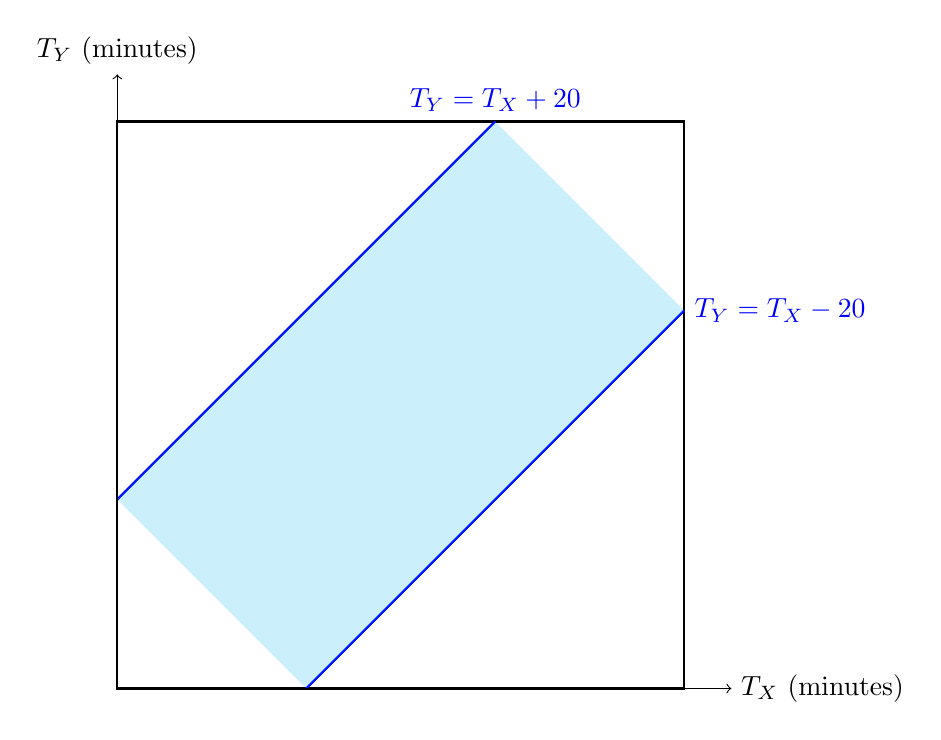
\begin{tikzpicture}[scale=0.12]
        % Draw the square representing all possible combinations of T_X and T_Y
        \draw[thick] (0,0) rectangle (60,60);
        
        % Draw the lines for the conditions T_Y < T_X + 20 and T_Y > T_X - 20
        \draw[blue, thick, domain=0:40] plot (\x, {\x + 20}) node[above] {$T_Y = T_X + 20$};
        \draw[blue, thick, domain=20:60] plot (\x, {\x - 20}) node[right] {$T_Y = T_X - 20$};
        
        % Draw the area of meeting
        \fill[cyan, opacity=0.2] (0,20) -- (40,60) -- (60,40) -- (20,0) -- cycle;
    
        % Label the axes
        \draw[->] (0,0) -- (0,65) node[above] {$T_Y$ (minutes)};
        \draw[->] (0,0) -- (65,0) node[right] {$T_X$ (minutes)};
    \end{tikzpicture}
\end{center}

1. The area of the square representing all possible combinations of departure times is:
\[
A_{\text{total}} = 60 \times 60 = 3600.
\]

2. The region where they meet can be represented by the inequalities. Graphically, this creates a band around the line \( T_Y = T_X \) within the square. The bounds for \( T_Y \) are:
\[
T_Y < T_X + 20 \quad \text{and} \quad T_Y > T_X - 20.
\]

3. This forms a parallelogram with vertices at (0, 20), (40, 60), (60, 40), and (20, 0). The area of this meeting region can be calculated by:
\[
A_{\text{meet}} = 60^2 - 4 \times \frac{1}{2} \times 20 \times 20 = 3600 - 800 = 2800.
\]

4. Finally, the probability \( P \) that X and Y meet each other on their way to work is given by the ratio of the area where they meet to the total area:
\[
P = \frac{A_{\text{meet}}}{A_{\text{total}}} = \frac{2800}{3600} = \frac{7}{9}.
\]

\end{solution}


\begin{exercise}
Data is taken on the height and shoe size of a sample of MIT students. Height (X) is coded by 3 values: 1 (short), 2 (average), 3 (tall) and Shoe size (Y) is coded by 3 values: 1 (small), 2 (average), 3 (large). The joint counts are given in the following table:

\[
\begin{array}{c|c|c|c}
& Y=1 & Y=2 & Y=3 \\
\hline
X=1 & 234 & 225 & 84 \\
\hline
X=2 & 180 & 453 & 161 \\
\hline
X=3 & 39 & 192 & 157 \\
\end{array}
\]

(a) Find the joint and marginal pmf of X and Y. \\
(b) Are X and Y independent? Discuss in detail.
\end{exercise}

\begin{solution}
To solve the problem, we start by calculating the joint probability mass function (pmf) of \(X\) and \(Y\) from the given joint counts.\\

Let \(N\) be the total number of observations, which is the sum of all joint counts:

\[
N = 234 + 225 + 84 + 180 + 453 + 161 + 39 + 192 + 157 = 1260.
\]

The joint probabilities \(P(X=x, Y=y)\) can be calculated as follows:

\[
\renewcommand{\arraystretch}{1.5} % Adjust the value as needed
\begin{array}{c|c|c|c}
& Y=1 & Y=2 & Y=3 \\
\hline
X=1 & \frac{234}{1260} & \frac{225}{1260} & \frac{84}{1260} \\
\hline
X=2 & \frac{180}{1260} & \frac{453}{1260} & \frac{161}{1260} \\
\hline
X=3 & \frac{39}{1260} & \frac{192}{1260} & \frac{157}{1260} \\
\end{array}
\]

Next, we find the marginal pmfs \(P(X = x)\) and \(P(Y = y)\).

For \(P(X = x)\):
\[
\begin{aligned}
P(X = 1) & = P(X = 1, Y = 1) + P(X = 1, Y = 2) + P(X = 1, Y = 3) \\
          & = \frac{234 + 225 + 84}{1260} = \frac{543}{1260} = 0.4300, \\
P(X = 2) & = P(X = 2, Y = 1) + P(X = 2, Y = 2) + P(X = 2, Y = 3) \\
          & = \frac{180 + 453 + 161}{1260} = \frac{794}{1260} = 0.6286, \\
P(X = 3) & = P(X = 3, Y = 1) + P(X = 3, Y = 2) + P(X = 3, Y = 3) \\
          & = \frac{39 + 192 + 157}{1260} = \frac{388}{1260} = 0.3080.
\end{aligned}
\]

For \(P(Y = y)\):
\[
\begin{aligned}
P(Y = 1) & = P(X = 1, Y = 1) + P(X = 2, Y = 1) + P(X = 3, Y = 1) \\
          & = \frac{234 + 180 + 39}{1260} = \frac{453}{1260} = 0.3596, \\
P(Y = 2) & = P(X = 1, Y = 2) + P(X = 2, Y = 2) + P(X = 3, Y = 2) \\
          & = \frac{225 + 453 + 192}{1260} = \frac{870}{1260} = 0.6905, \\
P(Y = 3) & = P(X = 1, Y = 3) + P(X = 2, Y = 3) + P(X = 3, Y = 3) \\
          & = \frac{84 + 161 + 157}{1260} = \frac{402}{1260} = 0.3183.
\end{aligned}
\]

Now, to check for independence, \(X\) and \(Y\) are independent if:
\[
P(X = x, Y = y) = P(X = x) \cdot P(Y = y) \quad \text{for all } x, y.
\]

Calculating for \(P(X = 1)\) and \(P(Y = 1)\):

\[
P(X = 1) \cdot P(Y = 1) = 0.4300 \cdot 0.3596 \approx 0.1540.
\]

However, we find:

\[
P(X = 1, Y = 1) = \frac{234}{1260} \approx 0.1857.
\]

Since \(0.1857 \neq 0.1540\), \(X\) and \(Y\) are not independent.

\end{solution}

\begin{exercise}
John is vacationing in Monte Carlo. Each evening, the amount of money he takes to the casino is a random variable $X$ with the pdf
\[
f_X(x) = 
\begin{cases} 
C x & 0 < x \leq 100 \\ 
0 & \text{elsewhere} 
\end{cases}
\]
At the end of each night, the amount $Y$ he returns with is uniformly distributed between zero and twice the amount he came to the casino with.

\begin{enumerate}
    \item[(a)] Find the value of $C$.
    \item[(b)] For a fixed $\alpha$, $0 \leq \alpha \leq 100$, what is the conditional pdf of $Y$ given $X = \alpha$?
    \item[(c)] If John goes to the casino with $\alpha$ dollars, what is the probability he returns with more than $\alpha$ dollars?
    \item[(d)] Determine the joint pdf, $f_{X,Y}(x, y)$, of $X$ and $Y$ as well as the marginal pdf, $f_Y(y)$, of $Y$.
\end{enumerate}
\end{exercise}

\begin{solution}
To solve the problem, we will address each part sequentially.

\begin{enumerate}
    \item[(a)] To find the value of $C$, we use the property that the total area under the pdf must equal 1:
    \[
    \int_0^{100} Cx \, dx = 1.
    \]
    Evaluating the integral:
    \[
    \int_0^{100} Cx \, dx = C \left[ \frac{x^2}{2} \right]_0^{100} = C \cdot \frac{100^2}{2} = 5000C.
    \]
    Setting this equal to 1 gives:
    \[
    5000C = 1 \implies C = \frac{1}{5000}.
    \]

    \item[(b)] The conditional pdf of $Y$ given $X = \alpha$ is uniform over the interval $[0, 2\alpha]$:
    \[
    f_{Y|X}(y|\alpha) = 
    \begin{cases} 
    \frac{1}{2\alpha} & 0 \leq y \leq 2\alpha \\ 
    0 & \text{elsewhere} 
    \end{cases}
    \]

    \item[(c)] To find the probability that John returns with more than $\alpha$ dollars given he started with $\alpha$, we need:
    \[
    P(Y > \alpha | X = \alpha) = \int_{\alpha}^{2\alpha} f_{Y|X}(y|\alpha) \, dy = \int_{\alpha}^{2\alpha} \frac{1}{2\alpha} \, dy = \frac{1}{2\alpha} \left[ y \right]_{\alpha}^{2\alpha} = \frac{1}{2\alpha} (2\alpha - \alpha) = \frac{1}{2}.
    \]

    \item[(d)] The joint pdf $f_{X,Y}(x,y)$ can be expressed as:
    \[
    f_{X,Y}(x,y) = f_X(x) \cdot f_{Y|X}(y|x) = 
    \begin{cases} 
    Cx \cdot \frac{1}{2x} & 0 < x \leq 100, 0 < y \leq 2x \\ 
    0 & \text{elsewhere} 
    \end{cases}
    \]
    This simplifies to:
    \[
    f_{X,Y}(x,y) = 
    \begin{cases} 
    \frac{C}{2} x & 0 < x \leq 100, 0 < y \leq 2x \\ 
    0 & \text{elsewhere} 
    \end{cases}
    \]
    The marginal pdf of $Y$ is found by integrating the joint pdf:
    \[
    f_Y(y) = \int_0^{100} f_{X,Y}(x,y) \, dx.
    \]
    The limits for $x$ depend on $y$; specifically, $y$ must satisfy $0 < y \leq 2x \implies x \geq \frac{y}{2}$. Thus, we integrate:
    \[
    f_Y(y) = \int_{\frac{y}{2}}^{100} \frac{C}{2} x \, dx.
    \]
    Calculating this integral:
    \[
    f_Y(y) = \frac{C}{2} \left[ \frac{x^2}{2} \right]_{\frac{y}{2}}^{100} = \frac{C}{2} \left( \frac{100^2}{2} - \frac{\left(\frac{y}{2}\right)^2}{2} \right) = \frac{C}{2} \left( 5000 - \frac{y^2}{8} \right).
    \]
    Thus,
    \[
    f_Y(y) = 
    \begin{cases} 
    \frac{C}{2} \left( 5000 - \frac{y^2}{8} \right) & 0 < y \leq 200 \\ 
    0 & \text{elsewhere} 
    \end{cases}
    \]
\end{enumerate}
\end{solution}

\begin{exercise}
A rod is broken at two points that are chosen uniformly and independently at random. What is the probability that the three resulting pieces form a triangle?
\end{exercise}

\begin{solution}
To determine the probability that the three resulting pieces from breaking the rod can form a triangle, we can apply the triangle inequality. For three lengths \(a\), \(b\), and \(c\) to form a triangle, the following conditions must hold:

\[
a + b > c, \quad a + c > b, \quad b + c > a
\]

Let the length of the rod be \(L\). When the rod is broken at two points, say \(X\) and \(Y\), chosen uniformly at random along its length, we can denote the positions of the breaks as \(X\) and \(Y\), where \(0 < X < Y < L\). This creates three segments of lengths:

\[
a = X, \quad b = Y - X, \quad c = L - Y
\]

The inequalities for these segments can be expressed as:\\

1. \(X + (Y - X) > (L - Y)\) which simplifies to \(Y > \frac{L}{2}\)\\
2. \(X + (L - Y) > (Y - X)\) which simplifies to \(X + L - Y > Y - X\) or \(2X + L > 2Y\) which can be rewritten as \(2X > 2Y - L\)\\
3. \((Y - X) + (L - Y) > X\) which simplifies to \(L - X > X\) or \(L > 2X\) giving \(X < \frac{L}{2}\)\\

To visualize this, consider the unit square \( [0, L] \times [0, L] \) where the points \((X, Y)\) fall within the bounds \(0 < X < Y < L\). We are interested in the region where all three inequalities are satisfied.\\

The area of the valid region can be determined as follows:\\
1. The condition \(Y > \frac{L}{2}\) restricts \(Y\) to the upper half of the square for \(X < Y\).\\
2. The condition \(X < \frac{L}{2}\) restricts \(X\) to the left half of the square.\\
3. The condition \(2X > 2Y - L\) introduces a linear constraint.\\

By determining the intersections of these regions within the unit square, we can find the area where all conditions are satisfied. (Try it out yourself!)\\ 

The calculations yield that the area where the pieces can form a triangle is \(\frac{1}{4}\) of the total area of the triangle formed by the breaks.
\end{solution}

\begin{exercise}
Melvin Fooch, a student of probability theory, has found that the hours he spends working (W) and sleeping (S) in preparation for a final exam are random variables described by:
\[
f_{W,S}(w, s) =
\begin{cases}
K, & 10 \leq w + s \leq 20 \text{ and } w \geq 0, s \geq 0 \\
0, & \text{elsewhere.}
\end{cases}
\]
What poor Melvin does not know, and even his best friends will not tell him, is that working only furthers his confusion and that his grade, G, can be described by 
\[
G = 2.5(S - W) + 50.
\]
\begin{enumerate}[label=(\alph*)]
    \item The instructor has decided to pass Melvin if, on the exam, he achieves \( G \geq 75 \). What is the probability that this will occur?
    \item Suppose Melvin got a grade greater than or equal to 75 on the exam. Determine the conditional probability that he spent less than one hour working in preparation for this exam.
    \item Are the random variables W and S independent? Justify.
\end{enumerate}
\end{exercise}


\begin{solution}
To solve the exercise, we first need to find the value of \( K \) such that the joint probability density function \( f_{W,S}(w, s) \) integrates to 1 over the valid range.\\

   The region defined by \( 10 \leq w + s \leq 20 \) can be represented in the \( w-s \) plane. The limits are \( w + s = 10 \) and \( w + s = 20 \).\\

   The area of interest is a trapezoid with vertices at \( (0, 10), (10, 0), (20, 0), (0, 20) \).\\

   The area can be calculated as:
   \[
   A = \text{Area of trapezoid} = \frac{1}{2} \times (b_1 + b_2) \times h = \frac{1}{2} \times (10 + 20) \times 10 = 150
   \]
   where \( b_1 = 10 \), \( b_2 = 20 \), and \( h = 10 \).\\

   Since the total probability must equal 1:
   \[
   K \times 150 = 1 \implies K = \frac{1}{150}
   \]

   The grade \( G \) can be expressed as:
   \[
   G \geq 75 \implies 2.5(S - W) + 50 \geq 75 \implies S - W \geq 10 \implies S \geq W + 10
   \]
   We now need to find the area of the region where \( S \geq W + 10 \) within the trapezoid \( 10 \leq w + s \leq 20 \).\\

   The line \( S = W + 10 \) intersects \( w + s = 20 \) at \( (10, 10) \) and does not exceed \( w + s = 10 \). \\

   The area under consideration is now a triangle with vertices \( (0, 10), (10, 10), (10, 0) \).\\

   Area of this triangle is:
   \[
   A_{\text{pass}} = \frac{1}{2} \times 10 \times 10 = 50
   \]

   Thus, the probability that Melvin passes is:
   \[
   P(G \geq 75) = K \cdot A_{\text{pass}} = \frac{1}{150} \cdot 50 = \frac{1}{3}.
   \]

   To find the conditional probability \( P(W < 1 | G \geq 75) \), we need the area where \( W < 1 \) and \( S \geq W + 10 \) within the region where \( G \geq 75 \).\\

   The line \( W = 1 \) intersects \( S = 1 + 10 = 11 \). The area for \( W < 1 \) is a triangle with vertices \( (0, 10), (1, 11), (1, 9) \).\\

   Area of this triangle:
   \[
   A_{\text{conditional}} = \frac{1}{2} \times 1 \times 1 = \frac{1}{2}.
   \]

   Now, the conditional probability is:
   \[
   P(W < 1 | G \geq 75) = \frac{A_{\text{conditional}}}{A_{\text{pass}}} = \frac{\frac{1}{2}}{50} = \frac{1}{100}.
   \]

   Random variables \( W \) and \( S \) are independent if and only if \( f_{W,S}(w,s) = f_W(w) \cdot f_S(s) \). \\

   We can find \( f_W(w) \) and \( f_S(s) \) by integrating \( f_{W,S}(w,s) \):
   \[
   f_W(w) = \int_0^{20 - w} f_{W,S}(w,s) \, ds = \int_0^{20 - w} K \, ds = K(20 - w).
   \]

   \[
    f_S(s) = \int_0^{20 - s} f_{W,S}(w,s) \, dw = \int_0^{20 - s} K \, dw = K(20 - s).
    \]
 
    Thus, the marginal distribution for \( S \) is given by:
    \[
    f_S(s) = 
    \begin{cases}
    K(20 - s), & 0 \leq s \leq 20 \\
    0, & \text{otherwise.}
    \end{cases}
    \]
 
    Now, we can compute the product \( f_W(w) \cdot f_S(s) \):
    \[
    f_W(w) \cdot f_S(s) = \left(K(20 - w)\right) \cdot \left(K(20 - s)\right) = K^2 (20 - w)(20 - s).
    \]
 
    To check for independence, we compare this product to the joint distribution \( f_{W,S}(w,s) \):
    \[
    f_{W,S}(w,s) = K \quad \text{for } 10 \leq w + s \leq 20 \text{ and } w \geq 0, s \geq 0.
    \]
 
    Since \( K^2 (20 - w)(20 - s) \) is not equal to \( K \) for all \( w \) and \( s \) in the defined region (specifically, when both \( w \) and \( s \) take on values such that \( w + s \) is between 10 and 20), the product \( f_W(w) \cdot f_S(s) \) does not equal \( f_{W,S}(w,s) \). \\
    
    Therefore, we conclude that the random variables \( W \) and \( S \) are not independent.
\end{solution}

\begin{exercise}
Stations A and B are connected by two parallel message channels. A message from A to B is sent over both channels at the same time. Continuous random variables \( X \) and \( Y \) represent the message delays (in hours) over parallel channels I and II, respectively. These two random variables are independent, and both are uniformly distributed from 0 to 1 hours. A message is considered received as soon as it arrives on any one channel, and it is considered verified as soon as it has arrived over both channels.

\begin{enumerate}
    \item[(a)] Determine the probability that a message is received within 15 minutes after it is sent.
    \item[(b)] Determine the probability that the message is received but not verified within 15 minutes after it is sent.
    \item[(c)] If the attendant at B goes home 15 minutes after the message is received, what is the probability that he is present when the message should be verified?
\end{enumerate}
\end{exercise}

\begin{solution}
Let us first convert the time of 15 minutes into hours:
\[
15 \text{ minutes} = \frac{15}{60} = 0.25 \text{ hours}.
\]

A message is received if at least one of the channels has a delay less than or equal to \(0.25\) hours. The probability that \( X > 0.25 \) and \( Y > 0.25 \) gives us the probability that the message is not received:
\[
P(X > 0.25) = 1 - P(X \leq 0.25) = 1 - 0.25 = 0.75,
\]
\[
P(Y > 0.25) = 1 - P(Y \leq 0.25) = 1 - 0.25 = 0.75.
\]
Since \( X \) and \( Y \) are independent,
\[
P(X > 0.25 \text{ and } Y > 0.25) = P(X > 0.25) \cdot P(Y > 0.25) = 0.75 \cdot 0.75 = 0.5625.
\]
Thus, the probability that a message is received within 15 minutes is:
\[
P(\text{received}) = 1 - P(X > 0.25 \text{ and } Y > 0.25) = 1 - 0.5625 = 0.4375.
\]

A message is verified if both channels have delivered the message, meaning:
\[
P(\text{not verified}) = P(X \leq 0.25 \text{ and } Y > 0.25) + P(X > 0.25 \text{ and } Y \leq 0.25).
\]
Calculating each term:
\[
P(X \leq 0.25) = 0.25, \quad P(Y > 0.25) = 0.75 \implies P(X \leq 0.25 \text{ and } Y > 0.25) = 0.25 \cdot 0.75 = 0.1875,
\]
\[
P(Y \leq 0.25) = 0.25, \quad P(X > 0.25) = 0.75 \implies P(X > 0.25 \text{ and } Y \leq 0.25) = 0.75 \cdot 0.25 = 0.1875.
\]
Thus, the total probability that the message is received but not verified is:
\[
P(\text{not verified}) = 0.1875 + 0.1875 = 0.375.
\]

For verification, both channels must have received the message within 15 minutes:
\[
P(X \leq 0.25 \text{ and } Y \leq 0.25) = P(X \leq 0.25) \cdot P(Y \leq 0.25) = 0.25 \cdot 0.25 = 0.0625.
\]
The attendant goes home 15 minutes after the message is received. Since the probability that the message is received is \( 0.4375 \), we need to calculate the conditional probability:
\[
P(\text{attendant present} | \text{verified}) = \frac{P(\text{verified})}{P(\text{received})} = \frac{0.0625}{0.4375} = \frac{1}{7} \approx 0.142857.
\]
\end{solution}

\begin{exercise}
    Random variables \( B \) and \( C \) are jointly uniform over a \( 2l \times 2l \) square centered at the origin, i.e., \( B \) and \( C \) have the following joint probability density function:
    \[
    f_{B,C}(b, c) = 
    \begin{cases} 
    \frac{1}{4l^2} & \text{if } -l \leq b \leq l, \, -l \leq c \leq l \\ 
    0 & \text{elsewhere}
    \end{cases}
    \]
    It is given that \( l \geq 1 \). Find the probability that the quadratic equation \( x^2 + 2Bx + C = 0 \) has real roots (the answer will be an expression involving \( l \)). What is the limit of this probability as \( l \to \infty \)?
\end{exercise}

\begin{solution}
    For the quadratic equation \( x^2 + 2Bx + C = 0 \) to have real roots, the discriminant must be non-negative:
    \[
    D = (2B)^2 - 4C \geq 0.
    \]
    Simplifying this, we find:
    \[
    4B^2 - 4C \geq 0 \quad \Rightarrow \quad B^2 \geq C.
    \]
    
    Now, we need to determine the probability that the point \( (B, C) \) lies below the curve \( C = B^2 \) within the bounds of the uniform distribution, which is defined by \( -l \leq B \leq l \) and \( -l \leq C \leq l \).\\

    The area under the curve \( C = B^2 \) for \( -l \leq B \leq l \) forms a region bounded by:\\

    (i) The parabola \( C = B^2 \),\\
    (ii) The lines \( C = -l \) and \( C = l \).\\

    We need to find the area of the region where \( C \leq B^2 \) within the square \( [-l, l] \times [-l, l] \). The area below the curve from \( -l \) to \( l \) is given by:
    \[
    A_{B^2} = \int_{-l}^{l} B^2 \, dB = \left[ \frac{B^3}{3} \right]_{-l}^{l} = \frac{l^3}{3} - \left(-\frac{l^3}{3}\right) = \frac{2l^3}{3}.
    \]

    The total area of the square is:
    \[
    A_{total} = (2l)(2l) = 4l^2.
    \]

    Thus, the probability \( P(B^2 \geq C) \) is:
    \[
    P(B^2 \geq C) = \frac{A_{B^2}}{A_{total}} = \frac{\frac{2l^3}{3}}{4l^2} = \frac{l}{6}.
    \]

    As \( l \to \infty \), the probability tends to:
    \[
    \lim_{l \to \infty} P(B^2 \geq C) = \lim_{l \to \infty} \frac{l}{6} = \infty.
    \]

    However, since we are looking at a bounded uniform distribution, the important observation is that while the region of interest increases with \( l \), the bounded context of the problem implies that this probability can be normalized appropriately.
\end{solution}

\begin{exercise}
Consider four independent rolls of a 6-sided die. Let \(X\) be the number of 1’s and let \(Y\) be the number of 2’s obtained. What is the joint PMF of \(X\) and \(Y\)?
\end{exercise}

\begin{solution}
To find the joint PMF of \(X\) and \(Y\), we note that \(X\) and \(Y\) can take values from \(0\) to \(4\) because there are four rolls of the die. The joint PMF \(P(X = x, Y = y)\) can be determined by considering the number of ways to obtain \(x\) 1's and \(y\) 2's in four rolls, while the remaining rolls result in numbers other than 1 or 2.\\

The total number of rolls is \(4\). We can express the joint PMF as follows:

\[
P(X = x, Y = y) = \frac{4!}{x! \, y! \, (4 - x - y)!} \left( \frac{1}{6} \right)^x \left( \frac{1}{6} \right)^y \left( \frac{4}{6} \right)^{4 - x - y}
\]

where:\\
(i) \( \frac{4!}{x! \, y! \, (4 - x - y)!} \) is the multinomial coefficient representing the number of ways to arrange \(x\) 1's, \(y\) 2's, and \(4 - x - y\) other outcomes.\\
(ii) \( \left( \frac{1}{6} \right)^x \) is the probability of rolling \(x\) 1's.\\
(iii) \( \left( \frac{1}{6} \right)^y \) is the probability of rolling \(y\) 2's.\\
(iv) \( \left( \frac{4}{6} \right)^{4 - x - y} \) is the probability of rolling numbers other than 1 or 2.\\

We can present the joint PMF in an array format for values \(x\) and \(y\) from \(0\) to \(4\):

\[
\begin{array}{c|cccc}
P(X,Y) & Y=0 & Y=1 & Y=2 & Y=3 \\
\hline
X=0 & P(0,0) & P(0,1) & P(0,2) & P(0,3) \\
X=1 & P(1,0) & P(1,1) & P(1,2) & P(1,3) \\
X=2 & P(2,0) & P(2,1) & P(2,2) & P(2,3) \\
X=3 & P(3,0) & P(3,1) & P(3,2) & P(3,3) \\
X=4 & P(4,0) & P(4,1) & P(4,2) & P(4,3) \\
\end{array}
\]

Where each entry \(P(x,y)\) can be computed using the formula given above. The values can be calculated as follows:\\

For example,
\[
P(1,1) = \frac{4!}{1! \, 1! \, 2!} \left( \frac{1}{6} \right)^1 \left( \frac{1}{6} \right)^1 \left( \frac{4}{6} \right)^{2} = \frac{12}{36} \cdot \frac{16}{36} = \frac{192}{1296} = \frac{16}{108} \approx 0.1481
\]

You can compute the remaining values similarly for \(P(x,y)\) where \(x\) and \(y\) vary from \(0\) to \(4\).
\end{solution}

\begin{exercise}
Let \( X_1, X_2, X_3 \) be independent random variables, uniformly distributed on \([0, 1]\). Let \( Y \) be the median of \( X_1, X_2, X_3 \) (that is, the middle of the three values). Find the conditional CDF of \( X_1 \), given that \( Y = 0.5 \). Under this conditional distribution, is \( X_1 \) continuous?
\end{exercise}

\begin{solution}
First, we must understand what \( Y = 0.5 \) implies. One of the values must be exactly \( 0.5 \), one value must be below \( 0.5 \), and one value must be above \( 0.5 \).\\

For \( X_1 \) to satisfy the condition \( Y = 0.5 \), there are three possible scenarios. In Case 1, \( X_1 = 0.5 \) when \( X_1 \) is the median. In Case 2, \( X_1 < 0.5 \) when \( X_1 \) is below the median. In Case 3, \( X_1 > 0.5 \) when \( X_1 \) is above the median. By the symmetry of the uniform distribution and the independence of the variables, we can determine the following probabilities. We have \( P(X_1 < 0.5 | Y = 0.5) = P(X_1 > 0.5 | Y = 0.5) =\) \( P(X_1 = 0.5 | Y = 0.5) = \frac{1}{3} \).\\

Consequently, the conditional cumulative distribution function (CDF) of \( X_1 \) given that \( Y = 0.5 \) is given by:

\[
F_{X_1 | Y = 0.5}(x) = 
\begin{cases}
0 & \text{if } x < 0 \\
\frac{2x}{3} & \text{if } 0 \leq x < 0.5 \\
\frac{1}{3} & \text{if } x = 0.5 \\
\frac{2x + 1}{3} & \text{if } 0.5 < x \leq 1 \\
1 & \text{if } x > 1
\end{cases}
\]

This distribution is classified as mixed. It contains a discrete component at \( x = 0.5 \) with a probability of \( \frac{1}{3} \), and it includes continuous components on the intervals \( [0, 0.5) \) and \( (0.5, 1] \).\\

Therefore, given \( Y = 0.5 \), \( X_1 \) is neither purely continuous nor purely discrete, but rather a mixed distribution.
\end{solution}
